% Propuesta inicial del proyecto final (1 página) - PDI 2026-2
% Compilar: pdflatex propuesta.tex
\documentclass[10pt]{article}
\usepackage[letterpaper,top=1.35cm,bottom=1.2cm,left=1.6cm,right=1.6cm]{geometry}
\usepackage[T1]{fontenc}
\usepackage[utf8]{inputenc}
\usepackage[spanish,es-noshorthands]{babel}
\usepackage{lmodern}
\usepackage{graphicx}
\usepackage{tabularx}
\usepackage{booktabs}
\usepackage{enumitem}
\usepackage{xcolor}
\usepackage{array}
\usepackage[hidelinks]{hyperref}

\definecolor{tinta}{HTML}{1B2430}
\definecolor{acento}{HTML}{1F5FA8}
\definecolor{gris}{HTML}{5A6270}
\pagestyle{empty}
\setlength{\parindent}{0pt}
\setlength{\parskip}{3pt}
\setlist{nosep,leftmargin=1.1em,topsep=1pt}
\renewcommand{\arraystretch}{1.12}

% sección numerada como en la guía del docente (01 ... 06)
\newcommand{\seccion}[2]{\par\vspace{7pt}{\color{acento}\sffamily\bfseries\small #1}\hspace{0.5em}{\color{tinta}\sffamily\bfseries #2}\par\vspace{1pt}}

\begin{document}
\color{tinta}

{\sffamily\footnotesize\color{gris} PROCESAMIENTO DIGITAL DE IMÁGENES · PROYECTO FINAL · PROPUESTA INICIAL}\\[2pt]
{\sffamily\bfseries\Large Detección de celdas solares defectuosas en imágenes de electroluminiscencia}\\[3pt]
{\small Johan Sebastián Cáceres Rodríguez · Hosman · Joel Eduardo Reyes Barrios \hfill
\color{gris}Repositorio: \texttt{solar-cell-el-defect-detection}}

\vspace{2pt}{\color{gris}\rule{\linewidth}{0.4pt}}

\begin{minipage}[t]{0.555\linewidth}
\seccion{01}{Problema y utilidad}
Las plantas solares y las fábricas de paneles revisan sus celdas con imágenes de \textbf{electroluminiscencia (EL)}: se inyecta corriente al panel en un cuarto oscuro y una cámara infrarroja capta la luz que emite cada celda. Las \textbf{microgrietas y zonas desconectadas} aparecen oscuras, no se ven a simple vista y reducen la potencia del panel. Revisar miles de celdas a ojo es lento y subjetivo. Es un problema de \textbf{inspección de calidad en electrónica y producción}, en la línea de los ejemplos del curso.

\seccion{02}{Objetivo y resultado}
Por cada celda, el sistema entrega:
\begin{enumerate}[label=(\arabic*),leftmargin=2em]
  \item el veredicto \textbf{FUNCIONAL / DEFECTUOSA} con su probabilidad;
  \item un \textbf{mapa de defectos} con las grietas y las zonas apagadas;
  \item \textbf{medidas}: \% de área apagada y longitud de las grietas.
\end{enumerate}
Como extras, el nivel de 4 clases del experto y un resumen por panel.
\end{minipage}\hfill
\begin{minipage}[t]{0.415\linewidth}
\seccion{03}{Imágenes}
Dataset público \textbf{ELPV} (ZAE Bayern / Univ. Erlangen-Nürnberg; Deitsch et al., \emph{Solar Energy}, 2019), con licencia CC BY-NC-SA 4.0 y acceso inmediato (\texttt{pip install elpv-dataset}). Contiene \textbf{2.624 celdas} de 300$\times$300\,px en gris, recortadas de \textbf{44 paneles} (18 mono y 26 policristalinos), cada una etiquetada por un experto: \textbf{1.803 funcionales} y \textbf{821 defectuosas}. Ya está descargado y analizado (EDA).

\vspace{4pt}
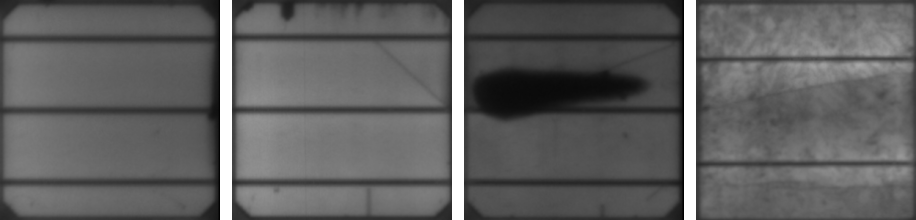
\includegraphics[width=\linewidth]{celdas_ejemplo.png}\\[-1pt]
{\scriptsize\color{gris}Sana (mono) · grieta (mono) · zona apagada (mono) · defecto (poli).}
\end{minipage}

\seccion{04}{Métodos de procesamiento}
\begin{tabularx}{\linewidth}{@{}>{\raggedright\arraybackslash}p{3.5cm}>{\raggedright\arraybackslash}X>{\raggedright\arraybackslash}p{3.3cm}@{}}
\toprule
\textbf{Etapa} & \textbf{Método y para qué} & \textbf{Tema del curso}\\
\midrule
Normalización & Dividir por el brillo propio de la celda (percentil) y CLAHE, porque cada panel se fotografió con distinta exposición. & Procesamiento por píxel\\
Máscara de la celda & Umbral, envolvente convexa y erosión para descartar bordes y esquinas. & Imágenes binarias, geometría\\
Quitar busbars y dedos & \textbf{Comparación de dos alternativas:} filtro \emph{notch} en el espectro de Fourier (son periódicos) frente a cierre morfológico con elemento lineal. & Fourier, morfología\\
Realzar defectos & Grietas con filtro de crestas (Hessiano/Sato) o Gabor; zonas apagadas con suavizado, déficit de brillo y umbral. & Filtrado, bordes\\
Mapa y medidas & Componentes conexas; área, longitud y orientación; descartar restos de busbar y granos (poli). & Descripción y geometría\\
Clasificación & Una sola \textbf{CNN pequeña} sobre la imagen ya procesada (3 canales: celda limpia, déficit, crestas). Inferencia opcional en la tarjeta Hailo. & Bloque de red\\
\bottomrule
\end{tabularx}

\begin{minipage}[t]{0.49\linewidth}
\seccion{05}{Forma de evaluación}
\textbf{Referencia:} la etiqueta del experto. \textbf{Partición por panel}, para que el sistema se mida con paneles que nunca vio:
\begin{itemize}
  \item ajuste: 30 paneles (1.790 celdas);
  \item validación: 7 paneles (432);
  \item prueba: 7 paneles (402).
\end{itemize}
Se verificó que no haya celdas casi idénticas entre partes.

\textbf{Métricas:} exactitud balanceada, F1 de la clase defectuosa, AUC y matriz de confusión, por separado para mono y poli. Además se mide el aporte del preprocesamiento (CNN con y sin él) y se compara con la literatura (82--88\%). Los errores se analizan caso por caso.
\end{minipage}\hfill
\begin{minipage}[t]{0.47\linewidth}
\seccion{06}{Alcance y recursos}
\textbf{Entregables:}
\begin{itemize}
  \item aplicación que recibe una celda y muestra las etapas intermedias, el mapa de defectos y el veredicto;
  \item código reproducible en GitHub;
  \item informe breve y sustentación.
\end{itemize}
\textbf{Recursos:} Python, OpenCV, scikit-image y PyTorch; GPU propia o Colab para entrenar; tarjeta Hailo (opcional).

\textbf{Fuera de alcance:} tomar imágenes EL propias (requiere cámara IR y cuarto oscuro) y segmentar el panel completo, porque el dataset ya trae las celdas recortadas. Las \emph{imágenes nuevas} de la demo son celdas de paneles de prueba.
\end{minipage}

\end{document}
